\documentclass[11pt,a5paper]{article}

\usepackage[T1]{fontenc}
\usepackage[utf8]{inputenc}
\usepackage{lmodern, microtype}
\usepackage[estonian]{babel}
%\usepackage[per=fraction, expproduct=cdot, decimalsymbol=comma, inter-unit-product=\cdot]{siunitx}
\usepackage{siunitx}
\sisetup{inter-unit-product=\ensuremath{{}\cdot{}}, per-mode=fraction, exponent-product=\cdot, output-decimal-marker={,}}
\usepackage{graphicx}
\usepackage{wrapfig}
\usepackage{subfig}
\usepackage{tikz}
\usetikzlibrary{arrows.meta}
\usepackage[european]{circuitikz}
\tikzset{component/.style={draw,thick,circle,fill=white,minimum size=0.75cm,inner sep=0pt}}
\usepackage{amsmath,amssymb}
\usepackage{amsfonts}
\usepackage{physics}
\usepackage[hidelinks]{hyperref}
\usepackage{csquotes}
\usepackage{caption}
\usepackage{enumitem}
\topmargin=-3.0cm \textheight=19cm \textwidth=12.9cm
\oddsidemargin=-1.5cm  \evensidemargin=-1.5cm
\setlength{\parindent}{0pt} \setlength{\parskip}{6pt} \sloppy
\sloppy \relpenalty=10000 \binoppenalty=10000
\pagestyle{empty}

\newcommand{\numb}[1]{\vspace{5pt}\textbf{\large #1}}
\newcommand{\nimi}[1]{(\textsl{\small #1})}
\newcommand{\punktid}[1]{(\emph{#1~p.})}
\newcounter{ylesanne}
\newcommand{\yl}[1]{\addtocounter{ylesanne}{1}\numb{\theylesanne.} \nimi{#1} \newblock{}}
%\newcommand{\autor}[1]{}% Kasuta võistluse ajal
\newcommand{\autor}[1]{\emph{ Autor: #1}}% Kasuta kui vaja autorit

\begin{document}
\begin{center}
  \textbf{\Large Eesti koolinoorte 34.\ füüsika lahtine võistlus} \par
  \emph{2.\ detsember 2023. a.\\Vanema rühma lahendused (11.--12.\ klass)}
\end{center}

\DeclareSIUnit\aasta{aasta}

\yl{PAVILJON}
\punktid{6} \autor{Uku Andreas Reigo}

Mõistame, et ülesande tingimustest tuletatav piiskade vertikaalne kiirus $v$ sõltub tuule suunast ruudukujulise paviljoni suhtes. Mõlemal korral vihmapiiskade horisontaalne nihe allpool katuseserva on $s = v_t T = \frac{v_t H}{v}$, kus $T$ on kukkumisaeg katuseservast põrandani. Esimesel juhul olgu tuule suund paviljoni mingi küljega risti:

\osa et 20\% põrandast märguks, peab piiskade horisontaalne nihe olema 20\% ruudu külje pikkusest.
\begin{align*}
    s = \frac{v_t H}{v} &= 0.2a \\
    \implies v &= \frac{v_t H}{0.2a} = \SI{9}{\meter\per\second}
\end{align*}

\osa Teine juht, tuule suund on piki ruudu diagonaali.

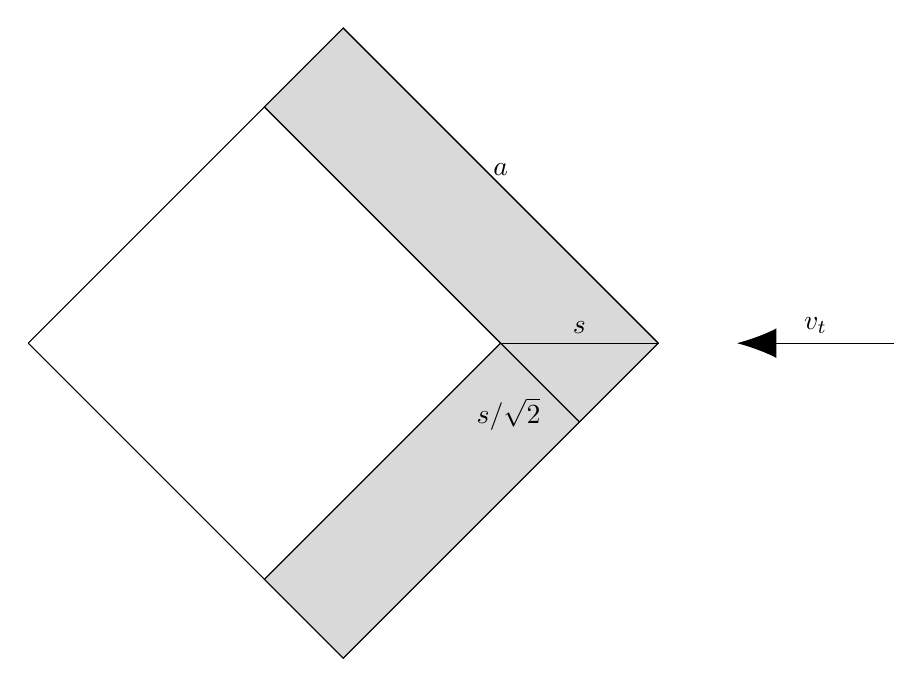
\begin{tikzpicture}[scale = 2]
    \draw (0,2) -- (2,0) --  (4,2)  -- (2,4) node[midway,above]{$a$}-- (0,2);
    \draw (1.5,3.5) -- (3,2) -- (1.5,0.5);
    \filldraw[fill=black!15](1.5,3.5)--(3,2)-- (1.5,0.5) -- (2,0) -- (4,2) -- (2,4) -- cycle;
    \draw (3,2) -- (4,2) node[midway,above]{$s$};
    \draw (3,2) -- (3.5,1.5) node[midway,xshift = -0.4cm, yshift = -0.4cm] {$s/\sqrt{2}$};
    \draw[-{Latex[length=5mm]}] (5.5,2) -- (4.5,2) node[midway,above]{$v_t$};
\end{tikzpicture}

Näeme, et kui kuiva ruudu külje pikkus on $b = a-\frac{s}{\sqrt{2}}$, ning kuiv ruut moodustab 80\% kogu ruudust, siis:

\begin{align*}
    b^2 &= (1-0.2)a^2\\
    \implies b &= \sqrt{0.8} a = a - \frac{s}{\sqrt{2}}\\
    \implies s &= \sqrt{2}(a-\sqrt{0.8}a) \\ 
    \implies v &= \frac{v_t H}{s} = \frac{v_t H}{\sqrt{2}(a-\sqrt{0.8}a)} \approx \SI{12}{\meter\per\second}
\end{align*}

Leiame, et minimaalne ja maksimaalne võimalik vihmapiisa kiirus on vastavalt $v_{min} = \SI{9}{\meter\per\second}$ ja $v_{max} = \SI{12}{\meter\per\second}$.


\yl{KUMERPEEGEL}
\punktid{6} \autor{Richard Luhtaru}

\begin{figure}[h]
    \centering
    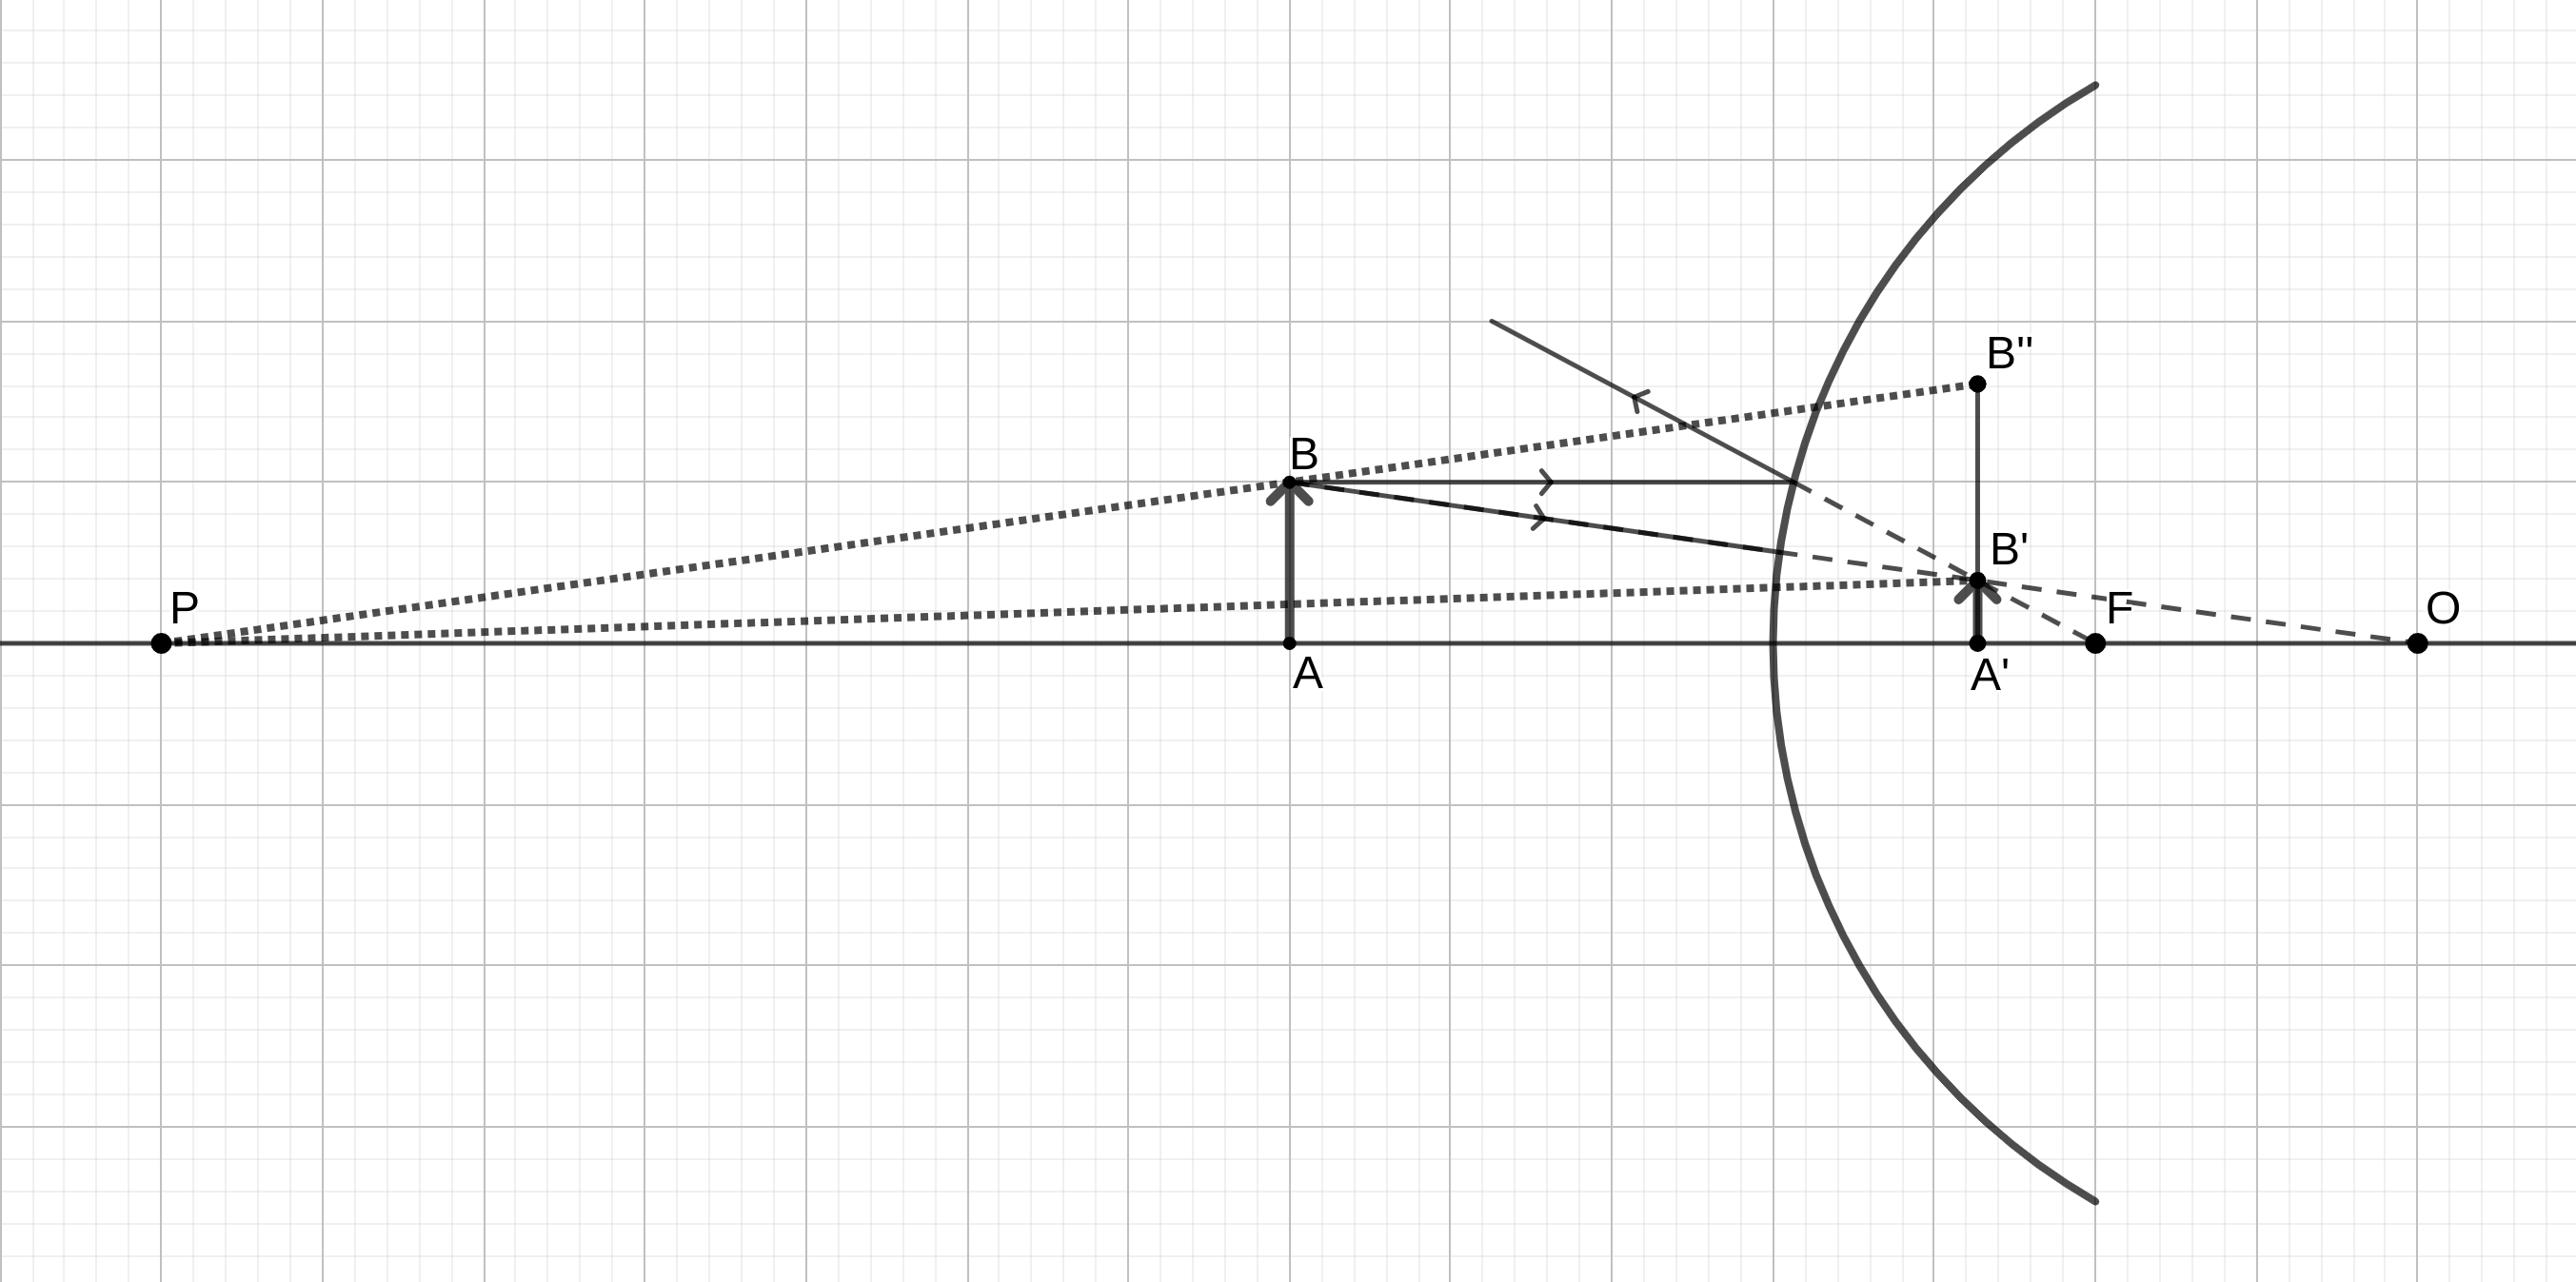
\includegraphics[width=\linewidth]{kumerpeegel-lah-joonis.png}
\end{figure}

Ese paistab kumerpeeglis sama suur, kui suur paistaks selle kujutis ilma kumerpeeglita. Leiame kõigepealt eseme AB kujutise A'B', tõmmates ühe kiire otse läbi punkti O ja teise kiire kõigepealt paralleelselt optilise peateljega ja seejärel läbi fookuse F.

Selleks, et leida kui palju paistab kujutis A'B' väiksem esemest AB, peame lisaks füüsilisele suurusele arvestama ka kaugusega. Jooniselt näeme, et näivate suuruste suhe on sama, mis on lõikude A'B' ja A'B'' suhe. Jooniselt hindame, et A'B' pikkus on 2 ruutu ja A'B'' pikkus on 8 ruutu. Seega kumerpeeglis paistab ese 4 korda väiksem.

\newpage

\yl{KUMMIPAEL}
\punktid{8} \autor{Valter Kiisk}

Esimese katse jaoks saame jõudude tasakaalutingimuse $k\Delta L=mg$, kus $k$ on kummipaela jäikustegur ja $m$ on koormise mass (mõlemad tundmatud). Siit saame avaldada suhte $mg/k=\Delta L$. Teises katses on kummipael juba algselt tugevasti deformeeritud olekus, kus tõmbejõud kummipaelas on $kL$ (sest pikkuse muut on $L$). Eeldame, et seetõttu läbivajumine $x\ll L$. Sel juhul, ühelt poolt, läbivajumisest tingitud kummipaela pikenemine on tühine ja seeläbi ka pinge paelas jääb peaaegu muutumatuks. Teiselt poolt, kummipael moodustab horisontaalsihiga nurga $\varphi\approx x/L$. Piki kummipaela suunatud jõu $kL$ projektsioon vertikaalsihile on siis ilmselt $kL\sin\varphi\approx kL\varphi\approx kx$. Kuivõrd kuumipaelal on nüüd kaks poolt, mis mõlemad ühtviisi panustavad koormise $mg$ tasakaalustamisse, siis $2kx=mg$, millest
\[
x =\frac{mg}{2k} =\frac{\Delta L}{2} = \SI{1}{cm}.
\]



\yl{KONDENSAATORID}
\punktid{8} \autor{Päivo Simson}

Enne laadimise algust on esimese kondensaatori energia
\[E_1=\frac{C_1U_0^2}{2}=4500\,\textrm{J}\]
ja teise energia on null. Laadimise käigus toimub kondensaatorite vahel laengu ümberjaotumine, kuid kogulaeng $q$ säilib. Laadimisprotsess toimub seni, kuni kondensaatorite pinged võrdsustuvad. Lõpp-pinge $U$ saame leida laengu jäävuse seadusest:
\[q=C_1U_0=C_1U+C_2U\quad\implies\quad U=\frac{C_1U_0}{C_1+C_2}=6\,\textrm{kV}.\]
Laadimise lõpuks on kahe kondensaatori koguenergia
\[E_2=\frac{C_1U^2}{2}+\frac{C_2U^2}{2}=\frac{(C_1+C_2)U^2}{2}=1800\,\textrm{J}.\]
Näeme, et see on väiksem kui esimese kondensaatori energia enne laadimise algust. Puuduolev energia eraldus järelikult süsteemist soojusena, peamiselt hõõglambi põlemisel. Otsitav soojushulk on seega
\[Q=E_1-E_2=2700\,\textrm{J}.\]
\emph{Märkus:} ülesande võib lahendada ka vahetulemusi kasutamata. Energia ja laengu jäävustest saame
\[
\begin{cases}
\displaystyle\frac{C_1U_0^2}{2}=\frac{C_1U^2}{2}+\frac{C_2U^2}{2}+Q\\
\,\,C_1U_0=C_1U+C_2U
\end{cases}
\implies Q=\frac{C_1C_2U_0^2}{2(C_1+C_2)}=2700\,\textrm{J}.
\]

\yl{ELEKTRIAUTO}
\punktid{10} \autor{Valter Kiisk}

\osa Autot kiirendav jõud avaldub võimsuse $P$ ja kiiruse $v$ kaudu: $F=P/v$. Graafikult on näha, et väikestel kiirustel $P$ kasvab võrdeliselt $v$-ga, nii et
\[
F=\frac{\SI{310}{\kilo\watt}}{\SI{65}{\kilo\meter\per\hour}}
\approx\frac{\SI{310000}{\watt}}{\SI{18}{\meter\per\second}}\approx\SI{17200}{\newton}
\]
Suurematel kiirustel $P$ jääb konstandiks või väheneb, seega maksimaalne veojõud ongi \SI{17200}{N} ja vastav kiirendus $a=F/m=\SI{7.8}{\meter\per\second\squared}$.

\osa Kuni kiiruseni $v_1=\SI{65}{\kilo\meter\per\hour}=\SI{18}{\meter\per\second}$ kulgeb auto ühtlase kiirendusega $a=\SI{7.8}{\meter\per\second\squared}$. Selle kiiruse saavutamiseks kulub aega
\[
t_1=\frac{v_1}{a}= \frac{\SI{18}{\meter\per\second}}{\SI{7.8}{\meter\per\second\squared}} \approx \SI{2.3}{s}.
\]
Suurematel kiirustel (kuni $v_2=\SI{100}{\kilo\meter\per\hour}$) mootori võimsus on konstant ($P=\SI{310}{\kilo\watt}$), seega kiirendus ajas muutub. Kiirenduse asemel on nüüd mugavam opereerida kineetilise energiaga. Kogu kasulik võimsus läheb auto kineetilise energia suurendamiseks, seega
\[
Pt_2=\frac{mv_2^2}{2} - \frac{mv_1^2}{2},
\]
millest
\[
t_2=\frac{m}{2P}(v_2^2-v_1^2)\approx \frac{\SI{2200}{\kilo\gram}}{2\cdot \SI{310000}{\watt}}\left[(\SI{28}{\meter\per\second})^2 - (\SI{18}{\meter\per\second})^2 \right]\approx \SI{1.6}{s}.
\]
Seega aega kulub kokku $t_1+t_2=\SI{3.9}{s}$.

\newpage

\yl{VÕIMAS MOOTOR}
\punktid{10} \autor{Marten Rannut}

Arvutame, mitu põlemistakti $N$ toimub mootoris 1 minuti jooksul. 4-taktilise mootori silindris toimub põlemistakt iga teine pööre ehk peame lisama konstandi $1/2$
$N = 1/2\cdot f n = 1/2\cdot \SI{8000}{\per\minute}\cdot 4= 16000$\\
Tulenevalt ideaalgaasi seadusest $V \cdot p = \frac{m}{\mu}RT$ (kus $V$ on gaasi ruumala, $p$ rõhk $m$ mass, $\mu$ molaarmass, $R$ universaalne gaasikonstant ja $T$ temperatuur) on gaasi tihedus $\frac{m}{V} = \frac{p\mu}{RT}$. Seega, kui gaasi tihedus temperatuuril $T_1$ on $\rho$, siis gaasi isobaarilisel soojendamisel temperatuurile $T_2$ muutub selle tihedus vastavalt valemile $\rho_2 = \rho \frac{T_1}{T_2}$. \\
Arvutame palju kütust $m$ põletab 1 põlemistakt, kui silindri maht on $v$.
$m = \rho_2v /\gamma  = \rho \frac{T_1}{T_2}v /\gamma  = \SI{1,2}{\gram\per\liter} \frac{\SI{293}{\kelvin}}{\SI{333}{\kelvin}} \SI{0,5}{\liter} / 14,7 \frac{g}{g} = \SI{0,036}{\gram}$

Kogu põletatud kütuse mass $M = N\cdot m = \SI{0,036}{\gram} * 16000 = \SI{576}{\gram}$

Arvutame mootori võimsuse  
$M \epsilon \eta \frac{1}{\SI{60}{\second}} = \SI{576}{\gram}\cdot\SI{46}{\kilo\joule\per\gram}\cdot 0,37\cdot \frac{1}{\SI{60}{\second}}=\SI{163}{\kilo\watt}$ 

Päris K20A mootori võimsus ongi umbes 162-165 kW olenevalt variandist.


\yl{SOOJUSPUMP}
\punktid{10} \autor{Jaan Kalda}

Oletame, et toa efektiivne soojusmahtuvus on $C$. Efektiivne soojusmahtuvus iseenesest ei pruugi olla üheselt mõistetav suurus, sest nt lühikese aja jooksul ei jõua seinte sügavamad osad veel soojeneda, mistõttu efektiivne soojusmahtuvus kasvab koos vaadeldava karakteerse ajavahemikuga. Antud juhul aga loodame, et karakteersed ajavahemikud --- $t_1$ ning hilisemas töörežiimis protsessi poolperiood --- tulevad samas suurusjärgus. Kui soojuspumba kütmisvõimsus on $P$, siis saame $Pt_1=C(T_1-T_0)$. Kui toa temperatuur on $T_f$, siis on ka soojuskadude võimsus $P_f$; üldjuhul on soojuskaod võrdelised sise- ja välistemperatuuride vahega, st soojuskadude võimsus $P_s=P(T-T_0)/(T_f-T_0)$. Nüüd saame välja kirjutada tingimused töörežiimis soojuspumba töötamise ($t_s$) ja puhkamise ($t_v$) ajavahemilke jaoks: $t_vP(T_k-T_0)/(T_f-T_0)=C(T_3-T_2)$ ning $t_s[P-P(T_k-T_0)/(T_f-T_0)]=t_sP(T_f-T_k)/(T_f-T_0)=C(T_3-T_2)$, kus $T_k=(T_3+T_2)/2=\SI{22}\celsius$ on toa keskmine temperatuur. Asendades $C$ esimesest võrrandist saame $$t_v=t_0\frac{T_3-T_2}{T_1-T_0}\frac{T_f-T_0}{T_k-T_0}=\SI{30}{\min}$$ ning $$t_s=t_0\frac{T_3-T_2}{T_1-T_0}\frac{T_f-T_0}{T_f-T_k}=\SI{30}\min.$$ Seega koguperiood $t_k=t_v+t_s=\SI{60}\min$.

\newpage

\yl{LÄÄTS}
\punktid{10} \autor{Valter Kiisk}

\osa Tähistame läätse raadiuse $r=\frac{1}{2}\cdot \SI{25.4}{mm}=\SI{12.7}{mm}$ (vt joonis). Läätse kumerpinnaga kaetud osa paksus on ilmselt $h = \SI{3.1}{mm} - \SI{2.0}{mm} = \SI{1.1}{mm}$. Nüüd Pythagorase teoreemi põhjal $R^2 = r^2 + (R - h)^2$, millest
\[
R = \frac{r^2 + h^2}{2h} = \frac{(\SI{12.7}{mm})^2 + (\SI{1.1}{mm})^2}{2\cdot \SI{1.1}{mm}}\approx \SI{73.8}{mm}.
\]

\osa Läätsele langevad paralleelsed kiired koonduvad fookuses. Õhukese läätse eeldusel võime fookuskauguseks lugeda lihtsalt fookuspunkti kauguse mistahes murdvast pinnast. Kõige lihtsam on seda analüüsi teha valguskiire jaoks, mis langeb läätsele vasakult, paralleelselt optilise peateljega. Seega esimesel pinnal murdumist ei toimu. Olgu langemisnurk kumerpinnale $\alpha$ ja murdumisnurk $\gamma$. Snelli seadusest $n\sin\alpha=\sin\gamma$. Kuna valguskiir eeldatavasti kulgeb optilise peatelje lähedal, siis kõik nurgad on väikesed, nii et $\sin\alpha\approx\alpha$ ja $\sin\gamma\approx\gamma$. Seega $\gamma\approx n\alpha$ ja $\varphi=\gamma-\alpha\approx(n-1)\alpha$. Langev kiir kulgeb optilisest teljest kaugusel $a=R\sin\alpha\approx \alpha R$. Samamoodi, pärast murdumist $\varphi f\approx a$ ehk
\[
f\approx\frac{a}{\varphi}=\frac{\alpha R}{(n-1)\alpha}=\frac{R}{n-1}\approx \SI{142}{mm}.
\]

\begin{center}
  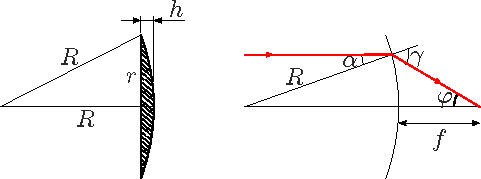
\includegraphics{tasakumer-laats-lah}
\end{center}

\yl{KLOTS JA SILINDER}
\punktid{12} \autor{Taavet Kalda}

Olgu nõlva kaldenurk $\alpha$ ning hõõrdetegur $\mu$.

Kuna silinder veeres libisemata, asus selle pöörlemiskese silindri ja mäenõlva kontaktpunktis. Vaatleme jõumomentide tasakaalu selle punkti suhtes. Kui silindri nurkkiirendus on $\epsilon$, siis
\[
I'\epsilon = mgR\sin\alpha,
\]
kus $I' = mR^2/2 + mR^2 = 3/2 mR^2$ on silindri inertsimoment kontaktpuntki läbiva telje suhtes (kasutades Steineri teoreemi). Silindri kiirendus on seega
\[
a_1 = R\epsilon = \frac{mR^2}{I'} \sin\alpha = \frac{2}{3}g\sin\alpha.
\]

Klotsi kiirendus allamäge takistab hõõrdejõud $mg\cos\alpha \mu$ ning kiirendab raskusjõud $mg\sin\alpha$. Klotsi kiirendus on seega
\[
a_2 = g\sin\alpha\mu - g\cos\alpha\mu.
\]
Peale silindri ja klotsi ühendamist hakkavad nad ühtse kehana mäest alla kiirenema kiirendusega $a_3$. Kui liigese pinge on $T$, siis silindrile mõjuvad jõud on raskuskiirendus, liigese pinge ning hõõrdejõu ja toereaktsiooni resultant. Kuna silinder ei libise, võime silindri jõumomentide tasakaalu jälle mäenõlva kontaktpunkti suhtes vaadelda (sest siis $a_3 = \epsilon / R$):
\[
I'\epsilon = mgR\sin\alpha + TR = I'\frac{a_3}{R}.
\]
Liigese pinge on seega
\[
T = \frac{3}{2}ma_3 - mg\sin\alpha.
\]
Klotsile mõjuvad sarnaselt liigese pinge, raskuskiirendus ning hõõrdejõu ja toereaktsiooni resultant. Mäenõlvaga paralleelne jõudude tasakaal esitub kujul
\[
ma_3 = mg\sin\alpha - T - mg\cos\alpha\mu = 2mg\sin\alpha - \frac{3}{2}ma_3 - mg\cos\alpha\mu.
\]
Seega,
\[
a_3 = \frac{4}{5}g\sin\alpha - \frac{2}{5}g\cos\alpha\mu.
\]
Näeme, et
\[
a_3 = \frac{2}{5}a_2 + \frac{3}{5}a_1.
\]
Ei tule suure üllatusena et tegu on kaalutud keskmisega, kus kiirendus on esimese ja teise stsenaariumite kiirenduste vahel.

Kui mäenõlva pikkus on $L$, siis kehtib $L = at^2/2$, st
\begin{align*}
t_3 &= \sqrt{\frac{2L}{a_3}} = \sqrt{\frac{2L}{\frac{2}{5}a_2 + \frac{3}{5}a_1}} = \sqrt{\frac{2L}{\frac{2}{5}\frac{2L}{t_2^2} + \frac{3}{5}\frac{2L}{t_1^2}}}\\
&= \sqrt{\frac{5}{2t_1^2+3t_2^2}}t_1t_2 = \SI{5.6}{s}.
\end{align*}

\pagebreak
\yl{KÕVER TRAJEKTOOR}
\punktid{12} \autor{Uku Andreas Reigo}

Et trajektoor on kinnine ja ülesanne on mitmes mõttes sümmeetriline (näiteks laengu ja algse suuna vahetamise korral peaks töötama, lisaks ka olukorra peegeldamisel üle sirge y=x), siis on näha, et nurk kiirusvektori ja x-telje vahel, kui elektron lahkub 1. veerandist, on samuti $\alpha$.

Edaspidi annan kõik nurgad positiivse x-telje suhtes vastupäeva mõõdetuna. 

%TODO korruta -1-ga, et tuleks positiivne osa ringist.
Algne nurk on $\theta_1 = \frac{\pi}{2} - \alpha$. 1. sektorist väljudes on nurk $\theta_2 = \alpha - \pi$, ehk $\Delta\theta = 2\alpha - \frac{3\pi}{2}$, seega sealne trajektoori osa moodustab $\frac{2\alpha-\frac{3\pi}{2}}{2\pi} = \frac{\alpha}{\pi} - \frac{3}{4}$ ringist. Järeldub ka, et kesknurk sisenemis- ja väljumispunkti vahel 1. sektoris on $\gamma = \frac{\pi}{2} + 2\alpha$

Samuti sümmeetriast teame, et trajektoor lõikab x-telge punktis $(h,0)$. Seega on sisenemis- ja väljumispunkti ühendava kõõlu pikkus $L = \sqrt{2}h$ ning ringi raadius $R_2 = \frac{L}{2\sin{\frac{\gamma}{2}}} = \frac{\sqrt{2}h}{2\sin{(\frac{\pi}{4}+\alpha)}}$



\begin{figure}[h]
    \centering
    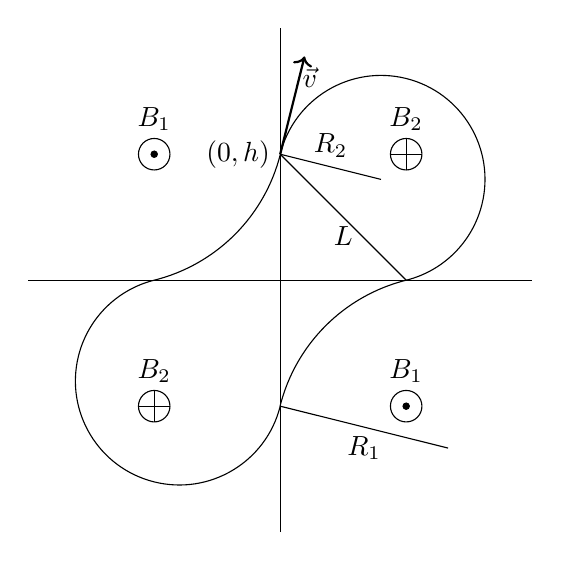
\begin{tikzpicture}[scale = 0.8]
        \draw (-4,0) -- (4,0);
        \draw (0,-4) -- (0,4);

        \draw[thick,->] (0,2) node [anchor = east] {$(0,h)$}
                            -- ++(76:1.6)
                            node [midway, yshift=10, anchor = west] {$\Vec{v}$};

        \draw (-2,2) circle (0.25) node[above, anchor = south, yshift = 5] {$B_1$};
        \filldraw (-2,2) circle (0.05);
        
        \draw (2,-2) circle (0.25) node[above, anchor = south, yshift = 5] {$B_1$};

        \filldraw (2,-2) circle (0.05);

        \draw (2,2) circle (0.25) node[above, anchor = south, yshift = 5] {$B_2$};
        \draw (2.25,2) -- (1.75,2);
        \draw (2,1.75) -- (2,2.25);

        \draw (-2,-2) circle (0.25) node[above, anchor = south, yshift = 5] {$B_2$};

        \draw (-2.25,-2) -- (-1.75,-2);
        \draw (-2,-1.75) -- (-2,-2.25);

        

        \draw (0,2) arc (166:-76:1.65);
        \draw (2,0) arc (104:166:2.75);
        \draw (0,-2) arc (-14:-256:1.65);
        \draw (-2,0) arc (-76:-14:2.75);

        \draw (0,2) -- (1.6,1.6) node[midway, above]{$R_2$};
        \draw (2.665,-2.665) -- (0,-2) node[midway, below]{$R_1$};
        \draw (0,2) -- (2,0) node [midway, below]{$L$};
    \end{tikzpicture}
    \caption*{Näidislahend $a = 14^\circ$ korral. $R_2 \approx 0.83 h$ ja $R_1 \approx 1.38 h$}
\end{figure}

2. sektoris viib sarnane arutelu arusaamani, et nurk muutub väärtuselt $\theta_2 = \alpha - \pi$ väärtuseni $\theta_3 = \frac{-\pi}{2} - \alpha$, läbides nurga $\Delta\theta = \frac{\pi}{2} - 2\alpha$. Seega kesknurk sisenemis- ja väljumispunkti vahel on $\gamma = \frac{\pi}{2} - 2\alpha$. Neid punkte ühendava kõõlu pikkus on jälle $L = \sqrt{2}h$ ning raadius $R_1 = \frac{L}{2\sin{\frac{\gamma}{2}}} = \frac{\sqrt{2}h}{2\sin{(\frac{\pi}{4}-\alpha)}}$

Et magnetväljas tiirleva elektroni tiirlemisraadius $R = \frac{mv}{qB}$, siis $\frac{R_1}{R_2} = \frac{B_2}{B_1} = \frac{\sin(\frac{\pi}{4}+\alpha)}{\sin{(\frac{\pi}{4}-\alpha)}}$ 


\end{document}